\section{Experiments}
\label{sec:exp}

The purpose of this experiment is to check how our generalized critic performs by comparison to a regular critic on top of a common actor, while paying a particular attention to the following factors:
\begin{enumerate}
\item the tasks, and whether different environments react differently to this change in implementation;
\item the hyperparameters of the advantage
\item the aggregation function, and how its parameters affect the average return.
\end{enumerate}

We will then provide the average total reward for each set of experiments and an interpretation of the results.

\subsection{Experiment Setting}
% In the case of a continuous action space, $\pi$ is a gaussian distribution. <- add this to experiments
For the sake of this experiment, we consider four continuous control tasks of the OpenAI Gym toolkit collection: 2D Walker, Inverted Pendulum, Ant and Half Cheetah. 

We implement our Generalized Critic on top of a Proximal Policy Optimization actor \cite{schulman2017proximal} of the clip variant, as given in \ref{subsec:po}.

The conducted experiments are as follows:
\begin{itemize}
\item A basic PPO with a regular critic will serve as a benchmark.
\item $\mathcal{F}_{phi_1}$ with two sets of generalized critic, each consisting in two advantage estimates.
\item $\mathcal{F}_{phi_2}$ with the same generalized critics.
\end{itemize}

For the sake of this experiment, $\phi_1$ and $\phi_2$ are both linear parameters such that $\mathcal{F}$ is a convex combination.

The two critics wil be characterized by the following hyperparameters:
\begin{description}
\item[$GC_1$] two advantage estimates with \lambda_1 = 0.98, \lambda_2 = 0.99, \gamma_1 = 0.99, \gamma_2 = 0.97
\item[$GC_2$] \lambda_1 = 0.98, \lambda_2 = 0.99, \gamma_1 = 0.99, \gamma_2 = 0.97
\end{description}

\subsection{Trained Tasks}

\subsection{Policy Optimization}
\label{subsec:po}
The policy optimization method that we use for this experiment is a Proximal Policy Optimization with the Clip variant.

%present ppo




\subsection{Experiment Results}

\begin{tabular}{p{14mm}p{14mm}p{15mm}p{11mm}p{14mm}}
Algorithm & 2D Walker & Inverted Pendulum & Ant & Half Cheetah\\
PPO (Base) & & & &  \\
\hline
$\lambda=0.1$, $\gamma=0.9$ & & & &  \\ 
\hline
$\lambda=0.1$, $\gamma=0.9$& & & &  \\ 
\hline
$\lambda=0.1$, $\gamma=0.9$& & & &  \\ 
\hline
$\lambda=0.1$, $\gamma=0.9$& & & &  \\
\end{tabular}


% Below is an example of how to insert images. Delete the ``\vspace'' line,
% uncomment the preceding line ``\centerline...'' and replace ``imageX.ps''
% with a suitable PostScript file name.
% -------------------------------------------------------------------------
\begin{figure}[htb]

\begin{minipage}[b]{1.0\linewidth}
  \centering
  \centerline{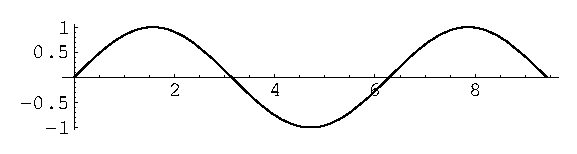
\includegraphics[width=8.5cm]{images/image1}}
%  \vspace{2.0cm}
  \centerline{(a) Result 1}\medskip
\end{minipage}
%
\begin{minipage}[b]{.48\linewidth}
  \centering
  \centerline{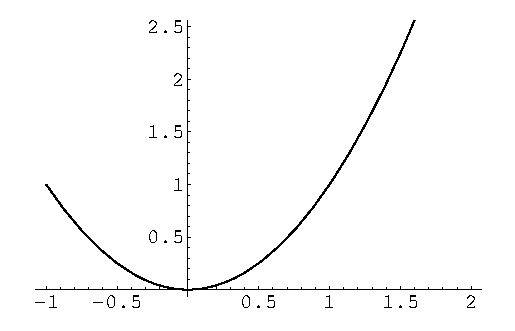
\includegraphics[width=4.0cm]{images/image3}}
%  \vspace{1.5cm}
  \centerline{(b) Results 3}\medskip
\end{minipage}
\hfill
\begin{minipage}[b]{0.48\linewidth}
  \centering
  \centerline{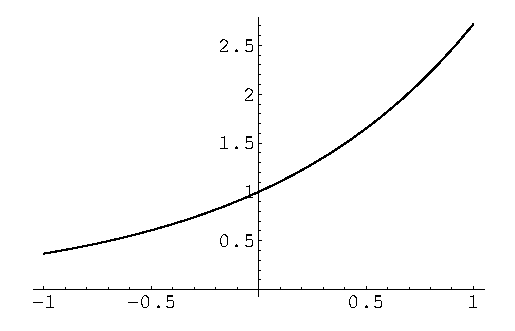
\includegraphics[width=4.0cm]{images/image4}}
%  \vspace{1.5cm}
  \centerline{(c) Result 4}\medskip
\end{minipage}
%
\caption{Example of placing a figure with experimental results.}
\label{fig:res}
%
\end{figure}


% To start a new column (but not a new page) and help balance the last-page
% column length use \vfill\pagebreak.
% -------------------------------------------------------------------------
%\vfill
%\pagebreak

